\documentclass[floatfix,nofootinbib,superscriptaddress,fleqn]{revtex4-2}  
%\documentclass[aps,epsfig,tightlines,fleqn]{revtex4}
\usepackage[utf]{kotex}
\usepackage[HWP]{dhucs-interword}
\usepackage[dvips]{color}
\usepackage{graphicx}
\usepackage{bm}
%\usepackage{fancyhdr}
%\usepackage{dcolumn}
\usepackage{defcolor}
\usepackage{amsmath}
\usepackage{amsfonts}
\usepackage{amssymb}
\usepackage{amscd}
\usepackage{amsthm}
\usepackage[utf8]{inputenc}
 \usepackage{setspace}
%\pagestyle{fancy}

\begin{document}

\title{\Large 2022년 1학기 물리학 I: Quiz 20}
\author{김현철\footnote{Office: 5S-436D (면담시간 매주
    화요일-16:00$\sim$20:00)}} 
\email{hchkim@inha.ac.kr}
\author{Lee Hui-Jae} 
\email{hjlee6674@inha.edu}
\affiliation{Hadron Theory Group, Department of Physics,
Inha University, Incheon 22212, Republic of Korea }
\date{Spring semester, 2022}


\vspace{1.cm}

\maketitle
\noindent {\bf 문제 1. (60 pt)} 
20 ${}^\circ\mathrm{C}$에서 강철자로
어떤 막대의 길이를 재었더니 정확하게 20.05 cm였다. 자와 막대를 270
${}^\circ\mathrm{C}$의 오븐에 넣고서 막대의 길이를 그 자로 재니까
20.11 cm였다. 막대를 이루고 있는 물질의 선팽창계수는 얼마인가? 
(강철의 선팽창계수는 $11\times 10^{-6}
\,({}^\circ\mathrm{C})^{-1}$이다.) 

\vspace{1.cm}

\noindent {\bf 풀이 :   }
온도가 $20\,\mathrm{^\circ C}$일 때 강철자의 길이를 $L_{st}$,
물체의 길이를 $L'$이라 하자.
선팽창계수를 고려하면 강철자가 늘어난 길이 $\Delta L_{st}$와
물체가 늘어난 길이 $\Delta L'$은
\begin{align}\label{eq:1-1}
  \Delta L_{st} =L_{st}\alpha_{st}\Delta T,\,\,\,
  \Delta L' =L'\alpha'\Delta T
\end{align}
이다. $\alpha_{st}$와 $\alpha'$은 각각 강철과 물체의 선팽창계수이다. 
강철자의 길이가 $20\,\mathrm{^\circ C}$에서 1 cm라고 생각해보자. 
오븐의 넣기 전 강철자로 잰 막대의 길이가 20.05 cm이므로
\begin{align}\label{eq:1-2}
  \frac{L'}{L_{st}} = \frac{20.05\,\mathrm{cm}}{1\,\mathrm{cm}}
  =20.05 \Longrightarrow L' = 20.05 L_{st}
\end{align}
이고 오븐에 넣고서 강철자로 잰 막대의 길이가 20.11 cm이므로
\begin{align}\label{eq:1-3}
  \frac{L'+\Delta L'}{L_{st}+\Delta L_{st}} = 20.11
  \Longrightarrow 
  L'+\Delta L' = (20.11)(L_{st}+\Delta L_{st})
\end{align}
이다. 식~\eqref{eq:1-1}과~\eqref{eq:1-2}를 식~\eqref{eq:1-3}에 대입하면
다음과 같다.
\begin{align}
  \begin{split}
    &L'(1+\alpha'\Delta T) = L_{st}(20.05)(1+\alpha'\Delta T)
    = L_{st}(20.11)(1+\alpha_{st}\Delta T)  \\
    &\Longrightarrow \alpha' = \frac{1}{\Delta T}\left(\frac{20.11}{20.05}
    (1+\alpha_{st}\Delta T)-1\right).
  \end{split}
\end{align}
따라서 물체의 열팽창계수 $\alpha'$는
\begin{align}
  \begin{split}
    \alpha' &= \frac{1}{250\,\mathrm{^\circ C}}\left(\frac{20.11}{20.05}
    \left(1+(11\times 10^{-6}\,\mathrm{^\circ C^{-1}})
    (250\,\mathrm{^\circ C})\right)-1\right)  \\
    &=2.3\times 10^{-5}\,\mathrm{^\circ C^{-1}}
  \end{split}
\end{align}
이다.

\vspace{1.cm}


\noindent {\bf 문제 2. (60 pt)}
어떤 물질의 비열이
\begin{align}
  \label{eq:1}
  c = 0.20 + 0.14 T + 0.023 T^2
\end{align}
으로 주어진다. 여기서 $T$는 섭씨온도이고 $c$의 단위는
cal/g$\cdot$K이다. 이 물질 2.0 g을 5.0 ${}^\circ\mathrm{C}$에서 15
${}^\circ\mathrm{C}$로 가열하는 데 필요한 에너지를 구하여라. 

\vspace{1.cm}
%%%%%%%%%%%%%%%%%%%%%%%%%%%%%%%%%%%%%%%%%%%%%%%%%%%%%%%%%%%%%%%%%%%%%%%%%%%%%%5
\noindent {\bf 풀이 :   }
비열이 $c$이고 질량이 $m$인 물질의 온도를 아주 작은 $dT$만큼 올리는데 필요한 에너지 $dQ$는
\begin{align}
 dQ = cm\,d T
\end{align}
이다. 이 물질의 온도를 $T_1$에서 $T_2$까지 가열한다고 할 때 필요한 에너지 $Q$는
\begin{align}
  \begin{split}
    Q &= m\int^{T_2}_{T_1}c\,dT
    = m \int^{T_2}_{T_1}0.20 +0.14T+0.023T^2\,dT  \\
    &= m\left( 0.20\left(T_2-T_1\right)+0.07\left(T_2^2-T_1^2\right)
    +\frac{0.023}{3}\left(T_2^3-T_1^3\right) \right)
  \end{split}
\end{align}
이다. $m$=2.0 g, $T_1$=5.0 $\mathrm{^\circ C}$이고 $T_2$=15 $\mathrm{^\circ C}$이므로
에너지 $Q$를 다음과 같이 얻는다.
\begin{align}
  \begin{split}
    Q &= (2.0\,\mathrm{g})\left(  
      (0.20)(10\,\mathrm{^\circ C})+(0.07)\left(
        (15\,\mathrm{^\circ C})^2-  
      (5.0\,\mathrm{^\circ C})^2\right)
      +\frac{0.023}{3}\left((15\,\mathrm{^\circ C})^3-  
      (5.0\,\mathrm{^\circ C})^3\right)
      \right) \\
      &= 82\,\mathrm{cal}.
    \end{split}
\end{align}
\vspace{1.cm}


\noindent {\bf 문제 3. (100pt) {\color{red}  (난이도 상)} }
질량이 50 g인 정육각형 얼음조각이 있다. 이 조각 두 개를 200 g의 물이
차 있는 단열통 안에 넣었다. 만약에 물의 처음 온도가 25
${}^\circ\mathrm{C}$이고, 냉동고에서 막 꺼낸 얼음조각의 온도는 $-15\,
{}^\circ\mathrm{C}$였다. 
\begin{itemize}
\item[(가)] 물과 얼음조각이 열평형에 이르렀을 때 온도는 얼마인가?
\item[(나)] 만약에 얼음조각을 하나만 넣었다면, 최종 온도는 얼마인가? 
\end{itemize}
\vspace{1.cm}
%%%%%%%%%%%%%%%%%%%%%%%%%%%%%%%%%%%%%%%%%%%%%%%%%%%%%%%%%%%%%%%%%%%%%%%%%%%%%%5
\noindent {\bf 풀이 :   }
\begin{itemize}
  \item[(1)]
  물과 얼음의 처음 온도를 $T_w$, $T_i$라 하고
물이 방출한 열을 $Q_{w}$, 얼음이 흡수한 열을 $Q_{i}$라고 하자.
$Q_{w}$과 $Q_{i}$는
\begin{align}
  \begin{split}
    Q_{w}  = c_{w}m_{w}\Delta T_w ,\,\,\,Q_{i} = c_{i}m_{i}\Delta T_i
  \end{split}
\end{align}
이다. 문제에 주어진 상황으로부터 열평형에 도달하면 가능한 열평형 상태는 세가지이다.
\begin{itemize}
  \item[1.] 모두 물이 된다.
  \item[2.] 모두 얼음이 된다.
  \item[3.] 물과 얼음이 공존하는 상태가 된다.  
\end{itemize}
세가지 중 어느 경우에 도달하는지 알아보자. 물이 방출한 열은 모두 얼음이 흡수하므로
$Q_{w}  =  Q_{i}$이고 열평형 온도를 $T_e$라고 하면
\begin{align}\label{eq:3-2}
  c_{w}m_{w}(T_w-T_e) = c_{i}m_{i}(T_e-T_i)
\end{align}
이다. 물과 얼음의 비열은 각각 $c_{w}=4.186\,\mathrm{J/g\cdot K}$,
$c_{i}=2.090\,\mathrm{J/g\cdot K}$임을 이용하면 $T_e$는
\begin{align}
  \begin{split}
    T_e &= \frac{c_i m_i T_i+c_w m_w T_w}{c_i m_i+c_w m_w}
    = \frac{(2.090\,\mathrm{J/g\cdot K}) (100\,\mathrm{g}) (-15\,\mathrm{^\circ C})
    +(4.186\,\mathrm{J/g\cdot K}) (200\,\mathrm{g}) (25\,\mathrm{^\circ C})}
    {(2.090\,\mathrm{J/g\cdot K}) (100\,\mathrm{g})
    +(4.186\,\mathrm{J/g\cdot K}) (200\,\mathrm{g})}  \\
    &= 17\,\mathrm{^\circ C}
  \end{split}
\end{align}
이다. 사실 이 답은 틀렸다. 얼음이 물로 상변이할 때 필요한 잠열을 고려하지 않았기 때문이다.
다만 이 결과를 통해 1번째 경우와 3번째 경우 중에 답이 있음을 알 수 있다. 
얼음이 물로 변하기 위해 필요한 잠열을 $L$이라고 하면 질량 $M$만큼의 얼음이 물로 변하기 위해
필요한 총 열 $Q_t$는
\begin{align}
Q_t = ML
\end{align}
이다. 물이 방출한 열이 상변이에 쓰이므로 식~\eqref{eq:3-2}는 다음과 같이 수정되어야한다.
\begin{align}
  Q_w = Q_i + Q_t
  \Longrightarrow c_{w}m_{w}(T_w-T'_e) = c_{i}m_{i}(T'_e-T_i)+ML.
\end{align}
$T'_e$는 새로운 열평형 온도이다.
3번째 경우는 간단하게 확인할 수 있으므로 $T'_e=0 ^\circ C$라고 해보자.
$L=3.33\times10^2\,\mathrm{J/g}$임을 고려하면 $M$은
\begin{align}
  \begin{split}
    M &= \frac{c_i m_i T_i+c_w m_w T_w}{L}
    = \frac{(2.090\,\mathrm{J/g\cdot K}) (100\,\mathrm{g}) (-15\,\mathrm{^\circ C})
    +(4.186\,\mathrm{J/g\cdot K}) (200\,\mathrm{g}) (25\,\mathrm{^\circ C})}
    {(3.33\times10^2\,\mathrm{J/g})}  \\
    &=53\,\mathrm{g}
  \end{split}
\end{align}
이다. 이는 열평형 온도가 $0 ^\circ C$이고 얼음이 53 g만큼 녹은 시점이라는 의미이다.

  \item[(2)] 
  (가)의 결과로부터 얼음 50 g이 사라지면 1번째 경우에 해당함을 알 수 있다. 얼음과
  물의 비열이 다르기 때문에, 얼음의 질량을 $m'_i$라 하여
  얼음 50 g이 0$^\circ C$가 되기까지 필요한 열 $Q_1$과 
  상전이에 필요한 열 $m'_iL$, 얼음이 녹은 물이 흡수한 열 $Q_2$를 모두 따져보자.
  열평형을 이루었을 때의 온도를 $T_f$라 하면
  \begin{align}
    Q_1 = c_i m'_i (0\,\mathrm{^\circ C} - T_i),\,\,\,
    m'_i L = m'_i(3.33\times10^2\,\mathrm{J/g}),\,\,\,
    Q_2 = c_w m'_i (T_f - 0\,\mathrm{^\circ C})
  \end{align} 
  이고 이 열들의 합은 물이 방출한 열 $Q'_w$와 같다. $Q'_w$는
  \begin{align}
    Q'_w = c_w m_w (T_w - T_f)
  \end{align}
  이다. 따라서
  \begin{align}
    Q'_w = Q_1+Q_2+m'_i L
  \end{align}
  이고 상평형 온도 $T_f$는
  \begin{align}
    c_w m_w (T_w - T_f) = -c_i m'_i T_i +c_w m'_i T_f + m'_i L
    \Longrightarrow
    T_f = \frac{c_w m_w T_w+c_i m'_i T_i-m'_i L}{c_w m_w+c_w m'_i}
  \end{align}
  이므로 계산해보면 $T_f$는
  \begin{align}
    \begin{split}
      T_f &= \frac{(4.186\,\mathrm{J/g\cdot K}) (200\,\mathrm{g}) 
      (25\,\mathrm{^\circ C})+(2.090\,\mathrm{J/g\cdot K}) (50\,\mathrm{g}) 
      (-15\,\mathrm{^\circ C})-(50\,\mathrm{g}) 
      (3.33\times10^2\,\mathrm{J/g})}
      {(4.186\,\mathrm{J/g\cdot K}) ((200\,\mathrm{g})+ (50\,\mathrm{g}))}  \\
      &= 2.6\,\mathrm{^\circ C}
    \end{split}
  \end{align}
  이다.
\end{itemize}
\vspace{1.cm}
\noindent {\bf 문제 4. (60pt)}
그림~\ref{fig:1}의 $p-V$
다이어그램에서처럼 순환경로 $abcd$를 따라 변하면서 기체가 한 일은
$+1.2$ J이었다. 경로 $ab$를 따라갈 때 내부에너지의 변화가 $+3.0$
J이고, 한 일의 크기는 5.0 J이며 경로 ca를 따라갈 때 기체로 전달된
열에너지는 $+2.5$ J이었다. 
\begin{figure}[ht]
  \centering
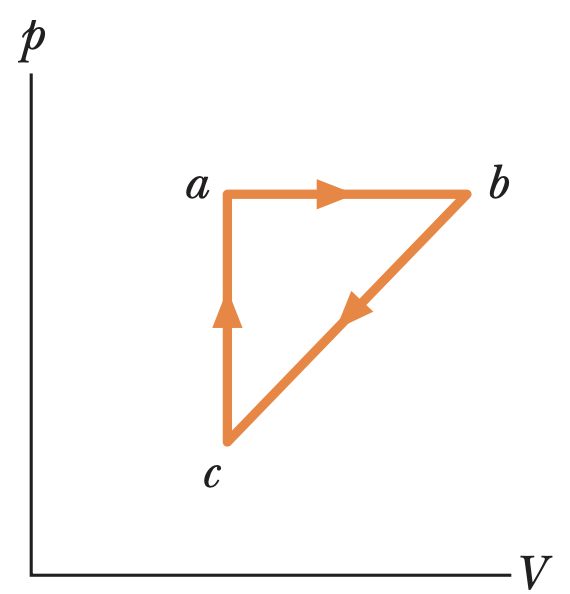
\includegraphics[scale=0.45]{Qfig21-1-20210525.png}
  \caption{문제 4}
  \label{fig:1}
\end{figure}
그렇다면
\begin{itemize}
\item[(가)] 경로 $ab$와
\item[(나)] 경로 $bc$를 따라갈 때 전달된 열에너지는 각각 얼마인가? 
\end{itemize}
\vspace{1.cm}
%%%%%%%%%%%%%%%%%%%%%%%%%%%%%%%%%%%%%%%%%%%%%%%%%%%%%%%%%%%%%%%%%%%%%%%%%%%%%%5
\noindent {\bf 풀이 :   }
열역학 제 1법칙은 다음과 같다.
\begin{align}\label{eq:4-1}
  dU = dQ -PdV.
\end{align}
\begin{itemize}
  \item[(가)]
  경로 $ab$는 등압과정, 경로 $ca$는 등적과정이다. 경로 $ab$를 거치면서 내부에너지가 
+3.0 J만큼 변하였고 외부에 5.0 J만큼 일을 해주었다. 식~\eqref{eq:4-1}에 의해 경로 $ab$를
다라가는 동안 기체에 전달된 열의 크기 $Q$는
\begin{align}
  Q = 3.0\,\mathrm{J} + 5.0\,\mathrm{J} 
  =8.0\,\mathrm{J}
\end{align}
이다. 
  \item[(나)] 전체 과정을 한번 순환하면 기체의 내부에너지의 변화는 없으므로  
  순환경로 $abca$를 한번 따라가면서 기체에 전달된 열에너지는 모두 기체가 외부에
  한 일로 변환된다. 기체에 전달된 열에너지의 합은
  \begin{align}
    Q_{ab}+Q_{bc}+Q_{ca} = 8.0\,\mathrm{J} +Q_{bc}+2.5\,\mathrm{J}
  \end{align}
  이고 기체가 외부에 한 일의 합은
  \begin{align}
    W_{ab}+W_{bc}+W_{ca} = 1.2\,\mathrm{J}
  \end{align}
  이다. 따라서 경로 $bc$를 따라갈 때 기체에 전달된 열에너지 $Q_{bc}$는
  \begin{align}
    Q_{bc} = 1.2\,\mathrm{J} - (8.0\,\mathrm{J} +2.5\,\mathrm{J})
    =-9.3\,\mathrm{J}
  \end{align}
  이다. $-$부호는 기체로부터 열에너지가 빠져나갔음을 의미한다.
\end{itemize}
\end{document}